\chapter{Theoretical Foundations}
\label{sec:theory}
This chapter will introduce important concepts for the reader. We start by introducing the rendering pipeline, then following into the development of more complex algorithms. We do not delve too deep in the implementations of the techniques discussed in this chapter - we provide a general understanding of the process in order to better situate the reader.

\section{The Rendering Pipeline}

In computer graphics, we say that the computer graphics pipeline is a model that describes the steps taken by a graphics system in order to render a 3D scene into a 2D screen (which is most often our computer monitors) \cite{Shreiner:2009}. This process is analogous to the way our eyes process the information around us and form images that are then processed by our brain and engraved into our minds.

Likewise, the computer must interpret some sort of description of an object or scene and pass this information through this pipeline into the final data format understood by our monitors. Most of the pipeline steps are implemented in hardware, allowing optimizations required for real-time rendering. 

A graphics pipeline can be divided into five core parts: 
\begin{enumerate}
 \item model and camera transformations
 \item lighting or shading
 \item projection
 \item clipping
 \item screen mapping
\end{enumerate}

Each individual part is essential to comprehend the workings of this pipeline. We, however, will be focusing our particular attention into the first two parts - \textit{model and camera transformations} and \textit{lighting}.

In part 1, the \textit{model and camera transformations}, we first process each object composing our scene and apply model transformations in order to position them in what is called the \textbf{world space}. The world space is defined by a coordinate system, a reference system to these objects in three-dimensional space.

With our scene now properly set, we then need to know how the camera - our eyes - is viewing the scene. Where is the camera? How far can the camera see? What is hidden from the camera? We need to represent the scene through the camera's reference system, which we call the \textbf{camera space}. Then, we can more easily determine which part of the scene will be within the camera's boundaries and discart the rest in order to improve performance.

In order to go from world space to camera space, one must apply camera transformations. Transforming from one to the other means one must change coordinate systems, which in Linear Algebra can be done by multiplying our models' coordinates (or vertexes) by a specific transformation matrix. 

In part 2, we must compute the amount of incident light in our objects, which will determine the color present at a given point. An earlier proposed way to compute lighting in the computer graphics pipeline was the \textit{Phong Reflection Model}. However, a lack of photorealism in the resulting images pushed for the development of more complex models for light interaction in the environment, such as the proposal of the \textit{Rendering Equation} and the creation of global illumination algorithms (\ie \textit{Ray Tracing} and \textit{MC Ray Tracing}).

\section{Phong Reflection Model}

The \textit{Phong Reflection Model} \cite{Phong:1975} was published as an empirical model of local illumination, describing how an object's surface reflects light as a combination of its material's properties - ambient, diffuse and specular reflection. This model can be represented by the following equation:

\begin{equation}
  I = k_a I_a + \sum_{m \in lights} (k_d (L \cdot N) + k_s (R \cdot V)^n) I_m
\end{equation}

where $k_a$, $k_d$ and $k_s$ represent, respectively, the ambient, diffuse and specular properties of the object; $L$ represents the direction of the incident light; $N$ represents the object's normal vector; $R$ represents the direction to which the incident light is reflected; $V$ represents the position from which we are observing the scene; and $I$ represents the incident light's intensity. This visual effects produced by this equation can be observed in Figure \ref{fig:phong}.

\begin{figure}[h]
  \centering
  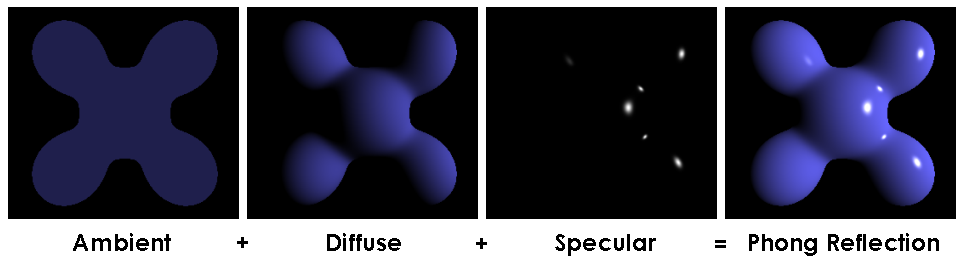
\includegraphics[width=\textwidth,height=\textheight,keepaspectratio]{images/3_theoretical_foundations/phong.png}
  \caption{Visual illustration of the Phong equation, extracted from \cite{wiki:phong}}
  \label{fig:phong}
\end{figure}

Phong's model was widely adopted: its efficiency proved to to be a deciding factor in generating real-time images for 3D scenes. The model, however, was unable to correctly represent global illumination. While the ambient term in the equation is a way of accounting for it, the term alone does not model physically-correct interactions between light and the environment. 

Algorithms that compute global illumination have a much higher computational cost, but produce more realistic images. One of the precursors of this type of algorithm was \textit{Ray Tracing}, which we  will review in our next section.

\section{Ray Tracing}

The \textit{Ray Tracing} algorithm \cite{Whitted:1980} consists of shooting rays from an imaginary "eye" (in this case, the camera) into the scene through a virtual screen. We trace the path of this ray until we find the closest object to intersect with it. Once the object has been identified, we - like in Phong Reflection Model - estimate the incoming light, examine the properties of the object and combine this information to determine the color in the output image. This process is illustrated in Figure \ref{fig:raytracing}.

\begin{figure}[h]
  \centering
  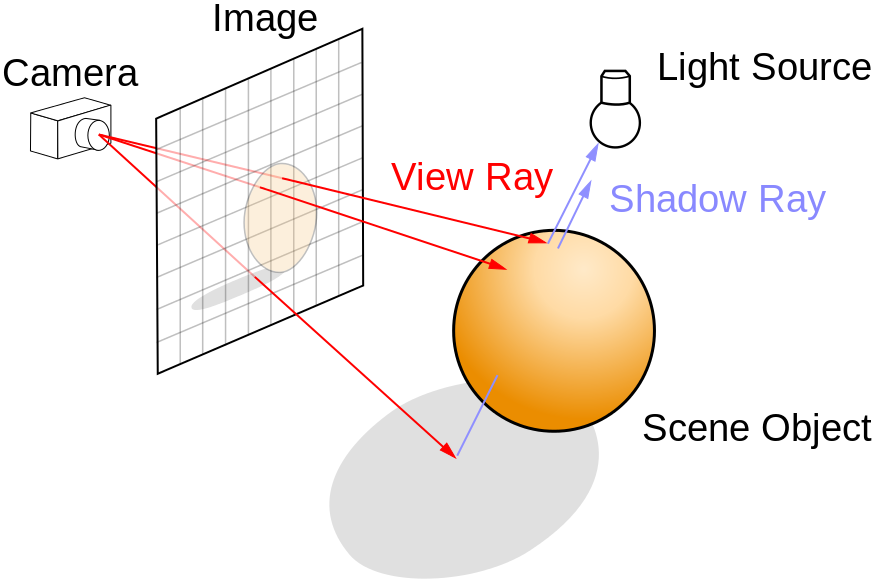
\includegraphics[width=0.45\textwidth,height=\textheight,keepaspectratio]{images/3_theoretical_foundations/raytracing.png}
  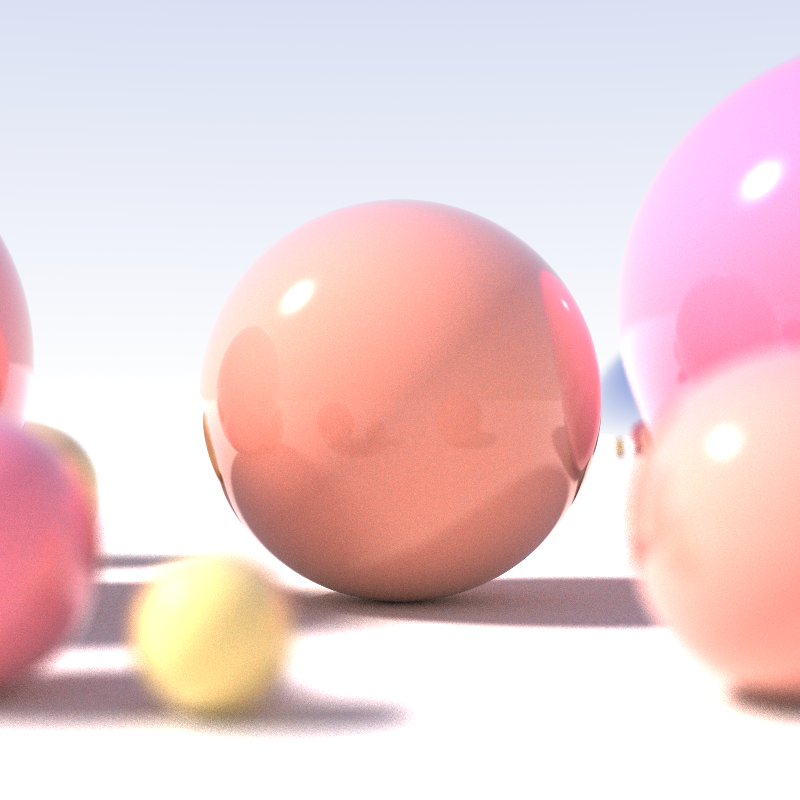
\includegraphics[width=0.45\textwidth,height=\textheight,keepaspectratio]{images/3_theoretical_foundations/raytracingexample.png}
  \caption{Visual illustration of the Ray Tracing algorithm (left) and an example of a scene rendered with the algorithm (right), extracted from \cite{wiki:raytracing}}
  \label{fig:raytracing}
\end{figure}

% While it may seem strange to send rays away from the camera - which is the opposite of how photographs are generated -, it is more cost-efficient as most light rays that incide on the scene do not reach the camera. Computing light paths is a strenuous task, and cutting back on this task load shortens the rendering time considerably.

The algorithm assumes that a surface may absorb some of the incident light, with results in a loss of intensity of the reflected light. This surface can also reflect the incident ray in more than one direction. If the object has translucent properties, the incident ray may be refracted, which results in an alteration of direction in the ray's path. These features mean that Ray Tracing, unlike its predecessors, is able to simulate a large selection of optical effects. 

It does not, however, come without disadvantages. In order to calculate the amount of light that arrives at an object, the most commonly used method is the Phong Reflection Model. This means that, while the algorithm creates a physically correct interaction of light rays with the environment, the final image is usually not photorealistic.

Photorealism can only be achieved when an algorithm approximates the \textit{Rendering Equation} - which describes every physical effect of light flow. This method will be furtherly discussed in our next section. 

\section{The Rendering Equation}

%The Rendering Equation \cite{Kajiya}
\red{WORK IN PROGRESS}

\subsection{Monte Carlo Ray Tracing}


